
% Note for any github stalkers. I am currently in the process
% of learning LaTeX. I don't know what I'm doing yet. Sorry
% if my code absolutely sucks.


\documentclass{book}

\usepackage{fontspec} % used to import Calibri
\usepackage{anyfontsize} % used to adjust font size

% needed for inch and other length measurements
% to be recognized
\usepackage{calc}

% for colors and text effects as is hopefully obvious
\usepackage[dvipsnames]{xcolor}
\usepackage{soul}

% control over margins
\usepackage[margin=1in]{geometry}
\usepackage[strict]{changepage}

\usepackage{mathtools}
\usepackage{amsfonts}
\usepackage{amssymb} % originally imported to get the proof square

% Just am using this to get a dashed line in a table...
% Also you apparently want this to be inactive if you aren't
% using it because it slows compilation.
\usepackage{arydshln} \ADLinactivate 
\newenvironment{allowTableDashes}{\ADLactivate}{\ADLinactivate}

\usepackage{graphicx}
%\graphicspath{{./140A_images/}}

\usepackage{tikz}
   \usetikzlibrary{arrows.meta}
   \usetikzlibrary{graphs, graphs.standard}

\newfontfamily{\calibri}{Calibri}
\setlength{\parindent}{0pt}
\definecolor{RawerSienna}{HTML}{945D27}


% Deprecated Text Commands (Don't use!!!)
% ~~~~~~~~~~~~~~~~~~~~~~~~~~~~~~~~~~~~~~~~~~~~~~~~~~~~
\newcommand{\hOneOld}{%
   \color{Black}%
   \fontsize{14}{14}\selectfont%
}
\newcommand{\hTwoOldd}{%
   \color{MidnightBlue}%
   \fontsize{13}{13}\selectfont%
}
\newcommand{\hThreeOld}{%
   \color{PineGreen}
   \fontsize{13}{13}\selectfont%
}
\newcommand{\hFourOldd}{%
   \color{Cerulean}
   \fontsize{12}{12}\selectfont%
}
\newcommand{\teachCommentOldd}{
   \color{Orange}%
   \fontsize{12}{12}\selectfont%
}
\newcommand{\exOneOldd}{%
   \color{Purple}%
   \fontsize{14}{14}\selectfont%
}
\newcommand{\exTwoOldd}{%
   \color{RedViolet}%
   \fontsize{13}{13}\selectfont%
}
\newcommand{\exPOldd}{%
   \color{VioletRed}%
   \fontsize{12}{12}\selectfont%
}
% Non Deprecated formatting commands use!!!
% ~~~~~~~~~~~~~~~~~~~~~~~~~~~~~~~~~~~~~~~~~~~~~~~~
\newcommand{\hOne}{%
   \color{Black}%
   \fontsize{14}{16}\selectfont%
}
\newcommand{\hTwo}{%
   \color{MidnightBlue}%
   \fontsize{13}{15}\selectfont%
}
\newcommand{\hThree}{%
   \color{PineGreen}
   \fontsize{13}{15}\selectfont%
}
\newcommand{\hFour}{%
   \color{Cerulean}
   \fontsize{12}{14}\selectfont%
}
\newcommand{\myComment}{%
   \color{RawerSienna}%
   \fontsize{12}{14}\selectfont%
}
\newcommand{\teachComment}{
   \color{Orange}%
   \fontsize{12}{14}\selectfont%
}
\newcommand{\exOne}{%
   \color{Purple}%
   \fontsize{14}{16}\selectfont%
}
\newcommand{\exTwo}{%
   \color{RedViolet}%
   \fontsize{13}{15}\selectfont%
}
\newcommand{\exP}{%
   \color{VioletRed}%
   \fontsize{12}{14}\selectfont%
}
% ~~~~~~~~~~~~~~~~~~~~~~~~~~~~~~~~~~~~~~~~~~~~~~~~

\newenvironment{myIndent}{%
   \begin{adjustwidth}{2.5em}{0em}%
}{%
   \end{adjustwidth}%
}

\newenvironment{myDindent}{%
   \begin{adjustwidth}{5em}{0em}%
}{%
   \end{adjustwidth}%
}

\newenvironment{myTindent}{%
   \begin{adjustwidth}{7.5em}{0em}%
}{%
   \end{adjustwidth}%
}

\newenvironment{myConstrict}{%
   \begin{adjustwidth}{2.5em}{2.5em}%
}{%
   \end{adjustwidth}%
}

\newcommand{\udefine}[1]{%
   \setulcolor{Red}%
   \setul{0.14em}{0.07em}%
   \ul{#1}%
}

\newcommand{\uuline}[2][.]{%
{\vphantom{a}\color{#1}%
\rlap{\rule[-0.18em]{\widthof{#2}}{0.06em}}%
\rlap{\rule[-0.32em]{\widthof{#2}}{0.06em}}}%
#2}

\newcounter{LectureNumber}
\newcommand*{\markLecture}[1]{%
   \stepcounter{LectureNumber}%
   {\huge \color{Black} \textbf{Lecture \theLectureNumber: #1} \newline}%
}

\newcommand{\pprime}{\prime\prime}

\newcounter{PropNumber}
\newcommand{\propCount}{%
   \stepcounter{PropNumber}%
   \thePropNumber%
}

\newcommand{\mySepOne}[1][.]{%
   {\noindent\color{#1}{\rule{6.5in}{1mm}}}\\%
}
\newcommand{\mySepTwo}[1][.]{%
   {\noindent\color{#1}{\rule{6.5in}{0.5mm}}}\\%
}

\newenvironment{myClosureOne}[2][.]{%
   \color{#1}%
   \begin{tabular}{|p{#2in}|} \hline \\%
}{%
   \\ \\ \hline \end{tabular}%
}

\newcommand{\retTwo}{\hfill\bigbreak}

\title{Math 158 Lecture Notes (Professor: Jacques Verstraete)}
\author{Isabelle Mills}


\begin{document}
   \maketitle
   \calibri

   \markLecture{1/9/2024}

   \hOneOld
   A \udefine{graph} is a pair $(V, E)$ where $V$ is a set of vertices
   and $E$ is a set of unordered pairs of elements of $V$ called edges.
   For $u, v \in V$, we say $u$ and $v$ are \udefine{adjacent} if 
   $\{u, v\} \in E$.

   
   \begin{center}
      \hTwoOldd
      For example: $G = (\{1, 2, 3\}, \{\{1, 2\}, \{2, 3\}\})$
      
      % I'm so sorry I'm not using the packages I should be using
      % to draw these graphs. I haven't had time to learn them yet
      % and I want this section done at some point tonight before I go
      % to bed. 
      \hThreeOld
      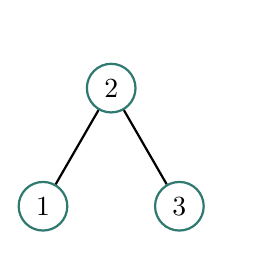
\begin{tikzpicture}
         \useasboundingbox (225:1.5) rectangle (45:2.5);

         \node (2) at (90:1) [circle, 
            draw=PineGreen!70!MidnightBlue, thick, fill=White] {2};
         \node (1) at (210:1) [circle, 
            draw=PineGreen!70!MidnightBlue, thick, fill=White] {1};
         \node (3) at (330:1) [circle, 
            draw=PineGreen!70!MidnightBlue, thick, fill=White] {3};
         \draw [thick] (1) -- (2);
         \draw [thick] (2) -- (3);
      \end{tikzpicture}
   \end{center}

\hOneOld
A \udefine{directed graph} (a.k.a a \udefine{digraph}) is a pair $(V, E)$ 
where $V$ is a set of vertices and $E$ is a set of ordered pairs 
of elements of $V$.
\begin{center}
   \hTwoOldd
   For example: $G = (\{1, 2, 3\}, \{(1, 2), (2, 3)\})$

   \hThreeOld
   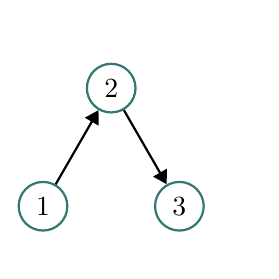
\begin{tikzpicture}
      \useasboundingbox (225:1.5) rectangle (45:2.5);

      \node (2) at (90:1) [circle, 
         draw=PineGreen!70!MidnightBlue, thick, fill=White] {2};
      \node (1) at (210:1) [circle, 
         draw=PineGreen!70!MidnightBlue, thick, fill=White] {1};
      \node (3) at (330:1) [circle, 
         draw=PineGreen!70!MidnightBlue, thick, fill=White] {3};
      \draw [thick, -Triangle] (1) -- (2);
      \draw [thick, -Triangle] (2) -- (3);
   \end{tikzpicture}
\end{center}

\hOneOld
A \udefine{multigraph} is a pair $(V, E)$ where $V$ is a set of vertices
and $E$ is a multiset of unordered pairs of elements of $V$.

\begin{center}
   \hTwoOldd
   For example: $G = (\{1, 2, 3\}, \{\{1, 2\}, \{2, 3\}, \{2, 3\}\})$
   
   \hThreeOld
   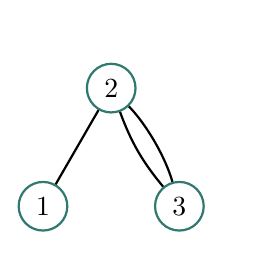
\begin{tikzpicture}
      \useasboundingbox (225:1.5) rectangle (45:2.5);

      \node (2) at (90:1) [circle, 
         draw=PineGreen!70!MidnightBlue, thick, fill=White] {2};
      \node (1) at (210:1) [circle, 
         draw=PineGreen!70!MidnightBlue, thick, fill=White] {1};
      \node (3) at (330:1) [circle, 
         draw=PineGreen!70!MidnightBlue, thick, fill=White] {3};
      \draw [thick] (1) -- (2);
      \draw [thick] (2) .. controls (50:.7) and (10:.7) .. (3);
      \draw [thick] (2) .. controls (50:.4) and (10:.4) .. (3);
   \end{tikzpicture}
\end{center}

\hOneOld
A \udefine{pseudograph} is like a graph and multigraph except that the
pairs in $E$ are multisets. 
\begin{myIndent}\begin{myIndent}\begin{myIndent}
\begin{myIndent}\begin{myIndent}
   \teachCommentOldd
   Essentially, an element $\{a, a\}$ can belong to $E$ in a 
   \\pseudograph. This type of edge is called a \udefine{loop}.
\end{myIndent}\end{myIndent}\end{myIndent}
\end{myIndent}\end{myIndent}

\begin{center}
   \hTwoOldd
   For example: $G = (\{1, 2, 3\}, \{\{1, 2\}, \{2, 3\}, \{3, 3\}\})$
   
   \hThreeOld
   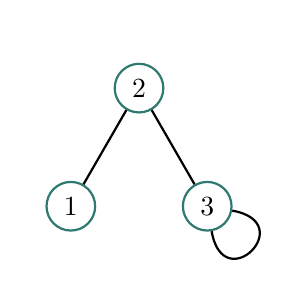
\begin{tikzpicture}
      \useasboundingbox (225:2) rectangle (45:2.5);

      \node (2) at (90:1) [circle, 
         draw=PineGreen!70!MidnightBlue, thick, fill=White] {2};
      \node (1) at (210:1) [circle, 
         draw=PineGreen!70!MidnightBlue, thick, fill=White] {1};
      \node (3) at (330:1) [circle, 
         draw=PineGreen!70!MidnightBlue, thick, fill=White] {3};
      \draw [thick] (1) -- (2);
      \draw [thick] (2) -- (3);
      \draw [thick] (3) to [out=350,in=280,looseness=6] (3);
   \end{tikzpicture}
\end{center}

\newpage
\hOneOld
If $G = (V, E)$ and $v \in V$, the \udefine{neighborhood} of $v$ is
$N_{G}(v)=\{w \in V \mid \{v, w\} \in E\}$. \bigbreak

The \udefine{degree} of $v$ is $d_{G}(v) = \lvert N_{G}(v) \rvert$.
Or in other words, $v$'s degree is equal to the number of edges 
connecting to $v$.

\mySepTwo[MidnightBlue]
\hTwoOldd
\begin{myIndent}
   The \udefine{Handshaking lemma} states that for any graph $(V, E)$:
      {\fontsize{16}{15}\selectfont
      \[ \sum_{v \in V} d_{G}(v) = 2 \lvert E \rvert \]}
   
   \hThreeOld
   \begin{myIndent}
      The reason for this is that each edge increments the degrees of
      exactly two vertices. So the above sum counts every edge twice.
      \hfill \bigbreak
   \end{myIndent}

   \hTwoOldd
   \uuline{Lemma}: Every graph has an even number of vertices with odd
   degrees.

   \hThreeOld
   \begin{myIndent}
      Proof: We can split the vertices of any graph into two categories:
      those with odd degrees, and those with even degrees.
      \hfill \bigbreak
      Now recall that an even number plus an even number always equals
      an even number, as does an odd number plus an odd number. However,
      an odd\\ number plus an even numbers equals an odd number. Based on
      this fact, we can guarentee that the sum of even degrees in any
      graph is even. And since the sum of even degrees plus the sum of 
      odd degrees must be even as it equals $2 \lvert E \rvert$ by
      the Handshaking lemma, we thus know that the sum of odd degrees 
      must be even. Hence, it must be the case that there are an even 
      number of vertices with odd degree because otherwise the sum of 
      their degrees won't be even.
      \hfill \bigbreak
   \end{myIndent}

   \hTwoOldd
   A graph is called \udefine{$r$-regular} if all of its vertices have
   degree $r$.
   \hThreeOld
   \begin{myIndent}
      Note that the number of edges in any $n$-vertex $r$-regular graph is
      $ \displaystyle{\frac{rn}{2}}$.
      \hfill \bigbreak
   \end{myIndent}
   
   \hTwoOldd
   An $r$-dimensional \udefine{cube graph}, denoted as $\mathrm{Q}_{r}$,
   is a graph such that $V(\mathrm{Q}_{r})$, the set of vertices in 
   $\mathrm{Q}_{r}$, is equal to the set of binary strings of 
   length $r$; and $E(\mathrm{Q}_{r})$, the set of edges in 
   $\mathrm{Q}_{r}$, is equal to the set of pairs of binary strings
   which differ in only one position.

   \begin{center}
      \begin{tabular}{ c c }
         \hThreeOld \fontsize{10}{10}\selectfont
         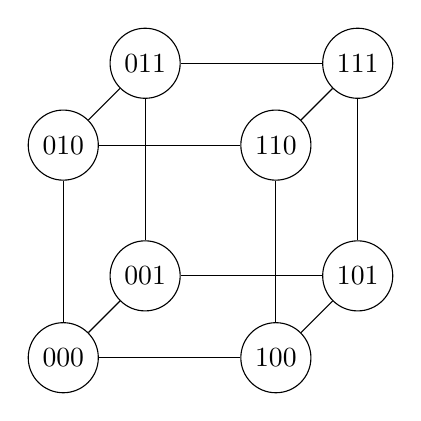
\begin{tikzpicture}[scale=0.9]
            \tikzstyle{myCir}=[circle,draw];
            \node[myCir] (000) at (0,0,0) {000};
            \node[myCir] (100) at (3,0,0) {100} edge (000);
            \node[myCir] (010) at (0,3,0) {010} edge (000);
            \node[myCir] (110) at (3,3,0) {110} edge (010) 
                                             edge (100);
            \node[myCir] (001) at (0,0,-3) {001} edge (000);
            \node[myCir] (101) at (3,0,-3) {101} edge (100) 
                                             edge (001);
            \node[myCir] (011) at (0,3,-3) {011} edge (010)   
                                             edge (001);
            \node[myCir] (111) at (3,3,-3) {111} edge (110) 
                                             edge (011) edge (101);
         \end{tikzpicture}
         & \hTwoOldd
         ${\displaystyle \quad\quad\quad
         \begin{matrix}
            \lvert V(\mathrm{Q}_{r})\rvert = 2^{r} \\ \\
            \lvert E(\mathrm{Q}_{r})\rvert = \frac{2^{r}r}{2} = 
               2^{r-1}r \\ \\ \\ \\{\teachCommentOldd\text{
                  Note that } \mathrm{Q}_{r} \text{ is } r
                  \text{-regular.}}
         \end{matrix}}$
      \end{tabular}
   \end{center}
\end{myIndent}

\newpage
\hOneOld
If $G=(V, E)$, then $H=(W, F)$ is a \udefine{subgraph} of $G$
if $W\subseteq V$ and $F\subseteq E$. \retTwo

If $W=V$, then $H$ is a \udefine{spanning subgraph} of $G$ (meaning 
that $H$ has the same vertices as $G$ but is lacking some of $G$'s 
edges) \retTwo

We define subtracting a set of vertices from a graph as follows:
\begin{myIndent} \hTwoOldd
   For $G = (V, E)$ and $X \subset V$, we define...
      \begin{myIndent}\begin{myIndent}
         ${\displaystyle G - X = (V \setminus X, \{\{u, v\}\in E 
         \mid \{u, v\}\cap X = \emptyset\}) }$
      \end{myIndent}\end{myIndent}
\end{myIndent}
\retTwo

\hOneOld % I might not actually need this command here...
We define subtracting a set of edges from a graph as follows:
\begin{myIndent} \hTwoOldd
   For $G = (V, E)$ and $L \subset E$, we define...
      \begin{myIndent}\begin{myIndent}\begin{myIndent}\begin{myIndent}
         ${\displaystyle G - L = (V, E \setminus L) }$
      \end{myIndent}\end{myIndent}\end{myIndent}\end{myIndent}
\end{myIndent} \retTwo

\hOneOld \markLecture{1/11/2024} \retTwo

We shall notate that $H$ is a subgraph of $G$ by 
writing $H \subseteq G$. \retTwo

An \udefine{induced subgraph} of $G = (V, E)$ is a subgraph 
$G\left[ X \right] = G - (V \setminus X)$ where $X \subseteq V$.
Alternatively, this is called the subgraph induced by $X$.
\retTwo

% Augh there is a bug with the uuline command I made!!!!
Given $G = (V, E)$ and $F \subseteq E$, the 
\udefine{subgraph spanned by $F$} is the subgraph whose edge set is $F$ 
and whose vertex set is ${\displaystyle
\bigcup_{e \in F}e}$. \retTwo

\mySepTwo \hOneOld
\begin{myIndent}\begin{myIndent}\begin{myIndent}\begin{myIndent}
   Here are some basic classes of graphs: \retTwo
\end{myIndent}\end{myIndent}\end{myIndent}\end{myIndent}

   \begin{itemize}
   \item \udefine{Complete graphs / cliques}, denoted $K_n$, are graphs 
      where every possible edge is present between $n$ vertices.\hTwoOldd

      \begin{center}
      \begin{allowTableDashes}\begin{tabular}
                           { c;{10pt/3pt}c;{10pt/3pt}c;{10pt/3pt}c c c }

         \begin{tikzpicture}[scale=0.5, inner sep=3pt]
            \useasboundingbox (-1.5,-3.5) rectangle (1.5,3);

            \tikzstyle{myCir}=[circle,fill];
            \node[myCir] (1) at (0:0) {};
            \node (name) at (270:3) {$K_1$};
         \end{tikzpicture}

         &

         \begin{tikzpicture}[scale=0.5, inner sep=3pt]
            \useasboundingbox (-3,-3.5) rectangle (3,3);

            \tikzstyle{myCir}=[circle,fill];
            \node[myCir] (1) at (0:2) {};
            \node[myCir] (2) at (180:2) {} edge (1);
            \node (name) at (270:3) {$K_2$};
         \end{tikzpicture}

         &

         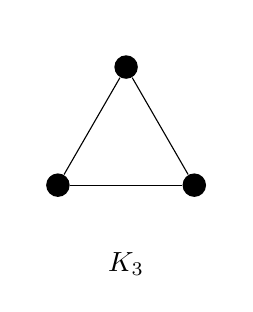
\begin{tikzpicture}[scale=0.5, inner sep=3pt]
            \useasboundingbox (-2.5,-3.5) rectangle (2.5,3);

            \tikzstyle{myCir}=[circle,fill];
            \node[myCir] (1) at (330:2) {};
            \node[myCir] (2) at (210:2) {} edge (1);
            \node[myCir] (3) at (90:2) {} edge (1) edge (2);
            \node (name) at (270:3) {$K_3$};
         \end{tikzpicture}

         &

         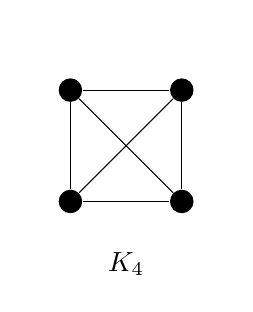
\begin{tikzpicture}[scale=0.5, inner sep=3pt]
            \useasboundingbox (-2.5,-3.5) rectangle (2.5,3);

            \tikzstyle{myCir}=[circle,fill];
            \node[myCir] (1) at (45:2) {};
            \node[myCir] (2) at (135:2) {} edge (1);
            \node[myCir] (3) at (225:2) {} edge (1) edge (2);
            \node[myCir] (4) at (315:2) {} edge (1) edge (2) edge (3);

            \node (name) at (270:3) {$K_4$};
         \end{tikzpicture}
      \end{tabular} \end{allowTableDashes}
      \end{center}

      
      \begin{myIndent}\begin{myIndent}\begin{myIndent}\begin{myIndent}
         \teachCommentOldd \begin{tabular}{ p{2.75in} c }
            
            Note we can also draw $K_4$ such that there are no edge
            interceptions as follows: &
         {\raisebox{-2.5em}{\tikz[scale=0.5, inner sep=3pt]{
            \tikzstyle{myCir}=[circle,fill];
            \node[myCir] (1) at (330:2) {};
            \node[myCir] (2) at (210:2) {} edge (1);
            \node[myCir] (3) at (90:2) {} edge (1) edge (2);
            \node[myCir] (4) at (0:0) {} edge (1) edge (2) edge (3);
         }}}
         \end{tabular}
      \end{myIndent}\end{myIndent}\end{myIndent}
      
      \hTwoOldd
      $\lvert V(K_n) \rvert = n$ \\
      $\lvert E(K_n) \rvert = \begin{pmatrix} n
         \vphantom{\frac{1}{1}} \\ 2\vphantom{\frac{
         \frac{1}{1}}{1}} \end{pmatrix} = \dfrac{n(n - 1)}{2}$ \retTwo
      \end{myIndent}
      \newpage

      \hOneOld
      \item A graph $G = (V, E)$ is bipartite if there exists a
         partition $(A, B)$ of $V$ such that every edge in $E$
         has one end in $A$ and one end in $B$. \retTwo
         {\hTwoOldd \begin{tabular}{p{2in} p{0.5in} p{3in}}
            \raisebox{-6em}{
               \tikz[scale=0.6, inner sep=3pt]{
                  \tikzstyle{myCir}=[circle, fill];

                  \draw[color=VioletRed, thick] 
                              (0, -1) arc (270:630:0.6 and 3);
                  \node (t) at (-1.25, 2) {{\color{VioletRed}\Huge A}};
                  
                  \draw[color=VioletRed, thick] 
                              (4, 0) arc (270:630:0.6 and 2);
                  \node (t) at (5.25, 2) {{\color{VioletRed}\Huge B}};
                  
                  \node[myCir] (t1) at (4,3) {};
                  \node[myCir] (t2) at (4,1) {};
                  \node[myCir] (s1) at (0,4) {} edge (t1) edge (t2);
                  \node[myCir] (s2) at (0,2) {} edge (t1);
                  \node[myCir] (s3) at (0,0) {} edge (t2); 
               }
            }
            &
            & 
            {The partition $(A, B)$ is called the \newline
            \udefine{bipartition} of $G$. Then $A$ and $B$ are called 
            the \udefine{parts} of $G$.}
         \end{tabular}} \retTwo

      \item A \udefine{Complete bipartite graphs} $K_{s,t}$, is the 
         bipartite graph with parts $A$ and $B$ where 
         $\lvert A \rvert = s$, $\lvert B \rvert = t$, and all 
         possible edges between $A$ and $B$ exist.

         \begin{myIndent}\begin{myIndent} \hTwoOldd
            For example, $K_{3,2}$: \hspace{2em} \raisebox{-2.3em}{
               \tikz[scale=0.5, inner sep=3pt]{
                  \tikzstyle{myCir}=[circle, fill];
                  \node[myCir] (t1) at (4,3) {};
                  \node[myCir] (t2) at (4,1) {};
                  \node[myCir] (s1) at (0,4) {} edge (t1) edge (t2);
                  \node[myCir] (s2) at (0,2) {} edge (t1) edge (t2);
                  \node[myCir] (s3) at (0,0) {} edge (t1) edge (t2); 
               }
            }
         \end{myIndent}\end{myIndent} \retTwo
   
      \item A \udefine{path} $P_k$ of length $k$ has a vertex set
         $V = \{v_1, v_2, \ldots, v_k, v_{k+1}\}$ and an edge set
         $E = \{\{v_1, v_2\}, \{v_2, v_3\}, \ldots, 
         \{v_{k-1}, v_k\}, \{v_k, v_{k+1}\}\}$.
      
         {\center \hTwoOldd
            Note that $\lvert V(P_k) \rvert = k+1$ and $\lvert E(P_k) 
            \rvert = k$. \\ Therefore, below would be $P_3$...
         
            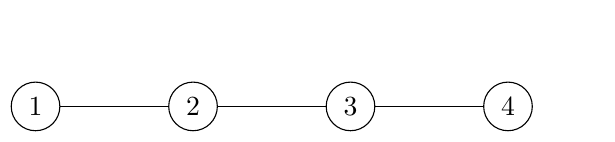
\begin{tikzpicture}
               \tikzstyle{myCir}=[circle, draw]

               \useasboundingbox (-0.1,-0.1) rectangle (7,1);

               \node[myCir] (4) at (6,0) {4};
               \node[myCir] (3) at (4,0) {3} edge (4);
               \node[myCir] (2) at (2,0) {2} edge (3);
               \node[myCir] (1) at (0,0) {1} edge (2);
            \end{tikzpicture} \retTwo
         
         \par }
      
      \item A \udefine{cycle} $C_k$ of length $k$ has a vertex set 
         $V = \{v_1, v_2, \ldots, v_k\}$ and an edge set $E = 
         \{\{v_1, v_2\}, \{v_2, v_3\}, \ldots, \{v_{k-1}, v_k\},
            \{v_k, v_1\}\}$.
         
         {\center \hTwoOldd
            Note that $\lvert V(C_k) \rvert = k$ and $\lvert E(C_k) 
            \rvert = k$. \\ Therefore, below would be $C_4$...

            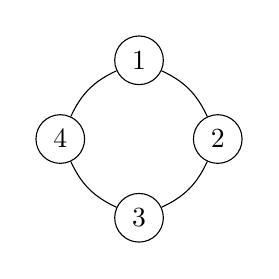
\begin{tikzpicture}[scale=0.5]
               \tikzstyle{myCir}=[circle, draw]

               \useasboundingbox (225:4) rectangle (45:4);

               \node[myCir] (2) at (0:2) {2};
               \node[myCir] (1) at (90:2) {1} edge [bend left=20] (2);
               \node[myCir] (4) at (180:2) {4} edge [bend left=20] (1);
               \node[myCir] (3) at (270:2) {3} edge [bend left=20] 
                        (4) edge [bend right=20] (2);
            \end{tikzpicture} \retTwo
         \par}

\end{itemize}
\newpage
Here is some terminology before the next lemma. For the graph
$G = (V, E)$\ldots
   
   \begin{itemize}
      \item $\delta(G) = \min\{d_G(v) \mid v \in V\}$ is the 
      \udefine{minimum degree} of $G$.
      \item $\Delta(G) = \max\{d_G(v) \mid v \in V\}$ is the 
      \udefine{maximum degree} of $G$.
      \item The \udefine{degree sequence} of $G$ is the 
      sequence of degrees of vertices $G$ in \\non-increasing order.
   \end{itemize}


\exOneOldd
\begin{center}
\begin{myClosureOne}{5.5}
   \uuline{Lemma (part 1)}: If $G = (V, E)$ is a graph of minimum degree
   $k \geq 2$, then $G$ contains a cycle of length at least
   $k + 1$.

   {\exPOldd \begin{myConstrict}
      Proof: Let $P$ be a longest possible path in $G$, say:
      \[V(P) = \{v_1, v_2, \ldots, v_r\}\]

      Then $N(v_r) \subseteq V(P)$. After all, if this were not 
      the case, we'd be able to extend the path to the vertex in 
      $N(v_r)$ but not in $V(P)$, thus contradicting the fact that
      $P$ is a longest path. \retTwo

      Let $v_i$ be the first neighbor of $v_r$ along the path from
      $v_1$ to $v_r$. Then $\{v_i, v_{i+1}, \ldots, v_r\}$ are the
      vertices of a cycle $C$. \retTwo

      Now note that because $N(v_r) \subseteq P$ and $v_i$ was
      the first element in the path $P$ to belong to $N(v_r)$, 
      we know that $C$ contains all the elements of $P$ that 
      $N(v_r)$ also has. So, $N(v_r) \subseteq C$. \retTwo

      But now note that $\lvert N(v_r) \rvert \geq \delta(G)=k$. Plus,
      $v_r$ itself is not in $N(v_r)$. Combining these facts together,
      we can say that the cycle $C$ has at least $k + 1$ vertices.
   \end{myConstrict}}

   \uuline{Lemma (part 2)}: The cycle length $k+1$ is the longest 
   we can guarentee based on the minimum degree of the graph being $k$.

   {\exPOldd \begin{myConstrict}
      Proof: Take the graph $K_{k+1}$ which has a minimum degree $k$. 
      \newline
      Obviously, the longest cycle in $K_{k+1}$ is the cycle containing
      all $k+1$ elements of $K_{k+1}$. Thus, we have shown that there
      are graphs with minimum degree $k$ which don't have cycles of
      length greater than \newline $k + 1$.
   \end{myConstrict}} 
\end{myClosureOne}
\end{center}
\retTwo

\hOneOld
A \udefine{connected graph} is a graph in which any two vertices
are the ends of a path. \retTwo

The \udefine{components} of a graph are the \uuline{maximal connected
subgraphs}. For example: \retTwo
{\hTwoOldd
   \begin{myIndent}\begin{myIndent}
      Let us define $G$ as: \hspace{2em}
      \raisebox{-2em}{\tikz[scale=0.4, inner sep=3pt]{
         \tikzstyle{myCir}=[circle, fill];
   
         \node[myCir] (t1) at (0, 1) {};
         \node[myCir] (t2) at (2, 1) {} edge (t1);
         \node[myCir] (t3) at (1, 3) {} edge (t1) edge (t2);
   
         \node[myCir] (y1) at (6, 2) {};
         \node[myCir] (y2) at (5, 4) {} edge (y1);
         \node[myCir] (y3) at (7, 4) {} edge (y1);
         \node[myCir] (y4) at (6, 0) {} edge (y1);
   
         \node[myCir] (p) at (10, 2) {};
   
         \draw[color=PineGreen, thick] 
                                 (-1.2, 2) arc (180:540:6 and 3);
      }} \retTwo

      As can be seen, $G$ has three components.
   \end{myIndent}\end{myIndent}
}
\newpage

A \udefine{tree} is a connected graph with no cycles
   (a.k.a it is acyclic). \hTwoOldd
   \begin{myIndent}
      Some examples of small trees include: $K_1$, $K_2$, $K_{1,2}$, 
      $P_3$, and $K_{1,3}$.
   \end{myIndent}

   \begin{center}
      \begin{myClosureOne}{5.5}
         \uuline{Lemma}: Every tree with $n$ vertices has exactly
         $n - 1$ edges.
         \hThreeOld
         \begin{myConstrict}
            Proof: We shall proceed by induction. \retTwo
            
            If $n = 1$, the tree is $K_1$, meaning that it has $0=n-1$
            edges. \retTwo

            Now assume the lemma is true for all trees with $n$
            vertices, and let $T$ be a tree with $n+1$ vertices. Then,
            we shall remove a vertex $v$ of $T$ with degree $1$. 
            (Note that we know such a vertex must exist since 
            otherwise the minimum degree of $T$ would be 
            at least $2$ and that would guarentee a cycle exists 
            of at least length 3. This
            of course contradicts the fact that $T$ is acyclic.)
            \retTwo 
            Then $T - \{v\}$ is a tree with $n$ vertices as it must be acyclic and connected. 
            So by induction it has $n-1$ edges. And because
            $v$ has degree $1$, we know that \newline $\lvert E(T) \rvert
            = 1 + \lvert E(T - \{v\}) \rvert = 1 + (n - 1) = n$.
         \end{myConstrict} \retTwo
         \hTwoOldd

         \uuline{Lemma}: Any connected graph with finite vertices has a spanning tree.
         \hThreeOld
         \begin{myConstrict}
            Proof: \retTwo

            Firstly consider the case that the graph $G$ has no cycle.
            Then, it is a tree by definition. \retTwo

            Now, consider if $G$ has a cycle $C$. Then for any edge \newline
            $e \in E(C)$, we have that $G - \{e\}$ is still connected.
            So, we can now go back to the top of the proof and ask:
            does $G -\{e\}$ have any cycles? We can repeatedly do this
            until the graph has no cycles since taking away edges
            does not remove any vertices.
            
         \end{myConstrict}
         \teachCommentOldd
         \begin{myIndent}\begin{myIndent}
            \begin{myConstrict}
            This actually acts as an algorithm for finding a spanning
            tree of any connected graph.
            \end{myConstrict}
         \end{myIndent}\end{myIndent}
      \end{myClosureOne}
   \end{center}\retTwo

\hOneOld

\begin{tabular}{ p{2in} p{1in} p{2.5in}}
   If $u$ and $v$ are two vertices in a connected graph, the
   \udefine{distance} from $u$ to $v$ is the length of a shortest
   path with ends at $u$ and $v$. & &
   \begin{centering} \hfill
      \raisebox{-6em}{\tikz[scale=0.9, inner sep=3pt, Black, very thick]{
            \tikzstyle{myCir}=[circle, fill];
            \tikzstyle{orng}=[color=Orange, line width=6pt, opacity=0.5];
      
            \node[myCir] (1) at (0, 0) {};
            \node[myCir] (2) at (2, 1) {} edge (1) edge[orng] (1);
            \node[myCir] (3) at (2, -1) {} edge (1) edge[orng] (1);
            \node[myCir] (4) at (3, 2) {} edge (2);
            \node[myCir, color=Red, label=above:{\color{red}$u$}] 
                  (5) at (4, .5) {} edge (2) edge[orng] (2);
            \node[myCir, color=Red, label=below:{\color{red}$v$}] 
                  (6) at (4, -.5) {} edge (3) edge[orng] (3);
            \node[myCir] (7) at (3, -2) {} edge (3);
            \node[myCir] (8) at (6, 1) {} edge (5);
            \node[myCir] (9) at (6, -1) {} edge (6);
         }}
   \end{centering}
\end{tabular}
\newpage

\hOneOld
Let $d_G(u, v)$ be the distance between $u$ and $v$.\retTwo

Distance is a \udefine{metric}, meaning:
\begin{myIndent}\begin{myIndent}\begin{enumerate}
   \item $d_G(u, v)=0 \Longleftrightarrow u=v$
   \item $d_G(u, v)=d_G(v, u)$
   \item $\forall w\in V, \hspace{0.5em}
      d_G(u, v) \leq d_G(u, w) + d_G(w, v)$
\end{enumerate}\end{myIndent}\end{myIndent} \retTwo

The \udefine{diameter} of a connected graph $G$ is the maximum distance
between any two vertices of $G$. Or in other words,
$\max\{d_G(u,v) \mid u,v\in  V(G)\}$. \retTwo

The \udefine{radius} of $G$ is equal to 
   $ \min\{\max\{d_g(u,v) \mid u\in V(G)\} \mid v\in V(G)\} $. What
   that means is that the radius of $G$ measures the smallest distance
   path one could limit themselves to drawing while still being able
   to have that path have one end at some fixed vertex and its other
   end at any arbitrary vertex in the graph.


\begin{myIndent}
   \hTwoOldd \uuline{Examples}:
   \begin{enumerate}
      \item The radius of $K_n$  is $1$. The diameter of $K_n$ is $n$.
      \retTwo
      \item The diameter of $P_k$ is $k$. The radius, can be computed as
         follows:
         \begin{myIndent} \hFourOldd
            The middle vertex of a path will have the fastest access
            to either end of the path. So, we shall measure the radius
            from the vertex: $v_{\lceil \frac{k+1}{2} \rceil}$. Then,
            we can see that $v_{k+1}$ is going to be a farthest element
            from $v_{\lceil \frac{k+1}{2} \rceil}$. So the radius
            of $P_k$ equals $k + \lceil \frac{k+1}{2} \rceil$.
            \retTwo

            Now you can consider what happens when $k$ is even and odd.
            But what's \\important is that it works out that the radius
            is $\lceil \frac{k}{2} \rceil$.
         \end{myIndent}
   \end{enumerate}
\end{myIndent} \retTwo
\hOneOld
We can use a \udefine{search tree} to more generally find
the radii and diameters of graphs. \retTwo

\begin{myIndent} \hTwoOldd
   \uuline{Breadth-First-Search}
   \begin{myIndent}
      Here's how to find a spanning tree in a connected graph with a root
      vertex $v$ such that the tree "preserves" all distances
      from $v$.
      (This tree is called a \udefine{BFS tree}).
      \begin{myIndent} \hThreeOld
         Let $G$ be a connected graph and let $(v_1, v_2, v_3,
         \ldots, v_n)$ be any ordering of the vertices of $G$.
         \retTwo
         Pick a vertex $v=v_1$ to be the root of the BFS tree.
         \retTwo
         Now, at any stage in constructing this tree, we will have
         a vertex set $V(T) = \{v_1, v_2 \ldots, v_k\}$ (when we first
         start, $V(T)$ will only contain $v_0$. So don't worry about that).
         Now if $V(T)=V(G)$ we can stop. Otherwise though, we can say 
         that there is a smallest integer $i$ such that for $v_i \in V(T)$, 
         $\hspace{0.25em} N(v_i)\setminus V(T) \neq \emptyset$.
         Choose $v_{k+1}$ to be the smallest neighbor (by the ordering of $V(G)$) of $v_i$ 
         not in $T$ and add 
         the edge $\{v_i, v_{k+1}\}$ to $T$. Then we repeat this paragraph.
         \retTwo
         Beware the ordering we are creating in our tree will often
         be different from the order of the graph you started with.
      \end{myIndent}
   \end{myIndent}
      \newpage
      \exOneOldd

      
   \begin{center}\begin{myClosureOne}{5.5}
      \uuline{Worked Demonstration}: \retTwo
      \exTwoOldd
      \begin{tabular}{ c c c }
         \begin{centering}
            \raisebox{-5em}{\tikz[scale=0.45,inner sep=4pt]{
               \tikzstyle{myCir}=[circle, draw];

               \node[myCir] (9) at (18:2) {9};
               \node[myCir] (7) at (90:2) {7};
               \node[myCir] (8) at (162:2) {8}
                  edge (9);
               \node[myCir] (3) at (234:2) {3}
                  edge (9) edge(7);
               \node[myCir] (10) at (306:2) {10}
                  edge (7) edge(8);
               \node[myCir] (5) at (18:5) {5}
                  edge (9);
               \node[myCir] (6) at (90:5) {6}
                  edge (7) edge (5);
               \node[myCir] (2) at (162:5) {2}
                  edge (6) edge (8);
               \node[myCir] (1) at (234:5) {1}
                  edge (2) edge (3);
               \node[myCir] (4) at (306:5) {4}
                  edge (1) edge (10) edge (5);
            }\par}
         \end{centering}
         &
         becomes
         &
         \begin{centering}
            \raisebox{-5em}{\tikz[scale=0.45,inner sep=4pt]{
               \tikzstyle{myCir}=[circle, draw];

               \node[myCir] (9) at (18:2) {9};
               \node[myCir] (7) at (90:2) {7};
               \node[myCir] (8) at (162:2) {8};
               \node[myCir] (3) at (234:2) {3}
                  edge (7) edge (9);
               \node[myCir] (10) at (306:2) {10};
               \node[myCir] (5) at (18:5) {5};
               \node[myCir] (6) at (90:5) {6};
               \node[myCir] (2) at (162:5) {2}
                  edge (6) edge (8);
               \node[myCir] (1) at (234:5) {1} 
                  edge (2) edge (3);
               \node[myCir] (4) at (306:5) {4}
                  edge (1) edge (5) edge (10);
            }\par}
         \end{centering}
      \end{tabular}
   \end{myClosureOne}\end{center} \retTwo

   \hTwoOldd
   \begin{myIndent}
      \uuline{Properties of BFS}: \hfill \bigbreak

      \begin{itemize}
         \item If the root is $v$, then $d_T(v, w) = d_G(v, w)$. In otherwords, a BFS tree \\preserves distances from its root. \newline
         
         \item The Tree with root $v$ has layers $N_i(v)=\{w\in V(G) \mid d_G(v, w)=i\}$. Furthermore all edges in the original graph either stay inside a single layer $N_i(v)$ or go between adjacent layers (i.e. from $N_i(v)$ to $N_{i+1}(v)$).
         {\begin{myIndent}\begin{myDindent}\begin{myDindent} \hThreeOld
            If an edge did "jump over" a layer, that \\violate the fact that distance is a metric. \newline
         \end{myDindent}\end{myDindent}\end{myIndent}}
         

         \item The diameter of $G$ equals the maximum number of
         layers of all BFS trees (not including the 0-layer). \newline

         \item The radius of $G$ equals the minimum number of layers
         of all BFS trees (also not including the 0-layer). \newline
      \end{itemize}
   \end{myIndent}
\end{myIndent}

\hOne
\mySepTwo \newline
\markLecture{1/16/2024}

Note that a tree is "minimally connecting" as subtracting any edge from a tree will produce a disconnected graph.
\begin{myIndent}
   We know this is the case because if we could remove an edge and still have the graph be connected, then that would imply the existence of a path between two neighboring vertices that doesn't go through their shared edge. But then, we'd be able to make a cycle subgraph by adding their shared edge to that path.
\end{myIndent}

\newpage

{\hTwo
\begin{myIndent}
   \uuline{Depth-First-Search}
   \begin{myIndent}
      Here is alternate algorithm for generating a spanning tree of a connected graph. A resulting tree of this algorithm is called a \udefine{DFS tree}.

      {\begin{myIndent} \hThree
         Let $G$ be a connected graph and let $(v_1, v_2, \ldots, v_n)$ be any ordering of the vertices of $G$. \retTwo

         Pick a vertex $v=v_1$ to be the root of the DFS-tree. \retTwo

         Now, at any stage in constructing this tree, we will have a vertex set $V(T)=\{v_1, v_2, \ldots, v_k\}$. If $V(T)=V(G)$, we can stop. Otherwise though, we select $i$ to be the largest integer such that for $v_i \in V(T)$,\\ $\hspace{0.25em} N(v_i)\setminus V(T) \neq \emptyset$. Then, choose $v_{k+1}$ to be the smallest neighbor (by the ordering of $V(G)$) of $v_i$ not in $V(T)$ and add 
         the edge $\{v_i, v_{k+1}\}$ to $T$. Then we repeat this paragraph.
         \retTwo
         Once again beware the ordering we are creating in our tree will typically be different from the order of the graph you started with. \retTwo
      \end{myIndent}}
   \end{myIndent}

   {\exOne
   \begin{center}\begin{myClosureOne}{5.5}
      \uuline{Worked Demonstration}: \retTwo
      \exTwoOldd
      \begin{tabular}{ c c c }
         \begin{centering}
            \raisebox{-5em}{\tikz[scale=0.45,inner sep=4pt]{
               \tikzstyle{myCir}=[circle, draw];

               \node[myCir] (3) at (4,2) {3};
               \node[myCir] (2) at (-4,2) {2}
                  edge (3);
               \node[myCir] (1) at (-4,-2) {1}
                  edge (2) edge (3);
               \node[myCir] (4) at (4,-2) {4}
                  edge (3) edge (2) edge (1);
               \node[myCir] (5) at (0,5) {5}
                  edge (2) edge (3);
               \node[myCir] (6) at (0,-5) {6}
                  edge (1) edge (4);
            }\par}
         \end{centering}
         &
         becomes
         &
         \begin{centering}
            \raisebox{-5em}{\tikz[scale=0.45,inner sep=4pt]{
               \tikzstyle{myCir}=[circle, draw];

               \node[myCir] (3) at (4,2) {3};
               \node[myCir] (2) at (-4,2) {2}
                  edge (3);
               \node[myCir] (1) at (-4,-2) {1}
                  edge (2);
               \node[myCir] (4) at (4,-2) {4}
                  edge (3);
               \node[myCir] (5) at (0,5) {5}
                  edge (3);
               \node[myCir] (6) at (0,-5) {6}
                  edge (4);
            }\par}
         \end{centering}
      \end{tabular}
   \end{myClosureOne}\end{center}} \hTwo\retTwo

   \mySepTwo[Black]

   \uuline{Theorem}: A graph is bipartite if and only if it contains no odd cycles.

   {\hThree
   \begin{myIndent}
      Proof: \\($\Longrightarrow$) First note that an odd cycle isn't bipartite. Thus, any graph containing an odd cycle is not bipartite. \retTwo

      ($\Longleftarrow$) Now supposed we are given some graph $G$ with no odd cycles. \\
      Then, assuming $G$ is connected (if $G$ isn't connected, we can break $G$ up into its component subgraphs and do this process for each component), we can construct a BFS-tree in $G$ rooted at some $v\in V(G)$. Let us name this tree $T$.
      \newpage

      Now as noted before, $T$ will have layers $L_i$ where each \\ $L_i=\{u\in V(G) \mid d_G(v, u)=i\}$. Using those layers, we can partition $T$ into two subsets $A$ and $B$ where $A$ is the union of all $L_i$ where $i$ is even and $B$ is the union of all $L_j$ where $j$ is odd. So, $T$ is clearly bipartite.
      \retTwo

      Now, let's reinsert the removed edges from $G$ back into $T$. Note that for each re-inserted edge $e$, it must be the case that either $e$ is a subset of some $L_i$ or that $e$ goes between some $L_i$ and $L_{i+1}$. Importantly, edges of the latter case do not violate our partition. So, if all the edges in $E(G) \setminus E(T)$ go between layers, then we can conclude that $G$ is definitely bipartite just like $T$.
      \retTwo

      With that, we now intend to show that an edge $G$ having an edge belonging to a single layer $L_i$ guarentees that $G$ contains an odd cycle.
      {\begin{myIndent} \hFour
         Assume the graph $G$ has an edge $\{u, w\}\subseteq L_i$ where $L_i$ is the $i$th layer of a BFS tree rooted at $v$. Then, we know that there exists a path $P_1$ contained in that BFS tree going from $v$ to $u$ and a path $P_2$ contained in that BFS tree going from $v$ to $w$. In order to draw a cycle from this information, let $x$ be the vertex of some $L_j$ such that $x\in V(P_1)$, $x\in V(P_2)$, and $j$ is as large as possible. That way, by defining the subpaths ${P_1}^\prime$ going from $x$ to $u$ and ${P_2}^\prime$ going from $x$ to $w$, we can get the following cyclic subgraph of $G$ :\[ C=(V({P_1}^\prime)\cup V({P_2}^\prime), E({P_1}^\prime)\cup E({P_2}^\prime) \cup \{u, w\})\]

         However, now note that $\lvert E({P_1}^\prime) \rvert = \lvert E({P_2}^\prime) \rvert = i-j$. Hence, \\$\lvert E(C) \rvert = 2(i-j)+1$, which in turn means that $C$ has an odd number of edges. So, we have shown that if a graph $G$ contains an edge within a single layer $L_i$, then we can give an example of an odd cycle within $G$. \retTwo
      \end{myIndent}}

      So in conclusion, if we assume $G$ has no odd cycles, then $G$ can't have any edges which are subsets of a single layer $L_i$. But that means that every edge in $G$ respects the partition we made to show that $T$ is bipartite. So, $G$ must also be bipartite with the same partition as $T$. $\blacksquare$
   \end{myIndent}
   }
\end{myIndent}}

\hOne
\mySepOne

A \udefine{Hamiltonian cycle} is a spanning cycle of a graph. We say a graph is \udefine{Hamiltonian} if it contains such a cycle. \retTwo

A \udefine{Hamiltonian path} is a spanning path of a graph. We say a graph is \udefine{traceable} if it has a hamiltonian path. \retTwo

A \udefine{walk} is a sequence of vertices and edges: i.e. $(v_1, \{v_1, v_2\}, v_2, \{v_2, v_3\}, ...)$

{\begin{myTindent} \teachComment
   Note that a walk can go over the same edge or vertex multiple times. \retTwo
\end{myTindent}}

A \udefine{trail} is a walk with no repeated edge.
{\begin{myTindent} \teachComment
   Interestingly, all paths are trails and all trails are walks. So a trail is kind of a middle concept between being a walk or a path.\retTwo
\end{myTindent}}
\newpage
A \udefine{tour} is a trail with the same first and last vertex.
{\begin{myTindent} \teachComment
   So, all cycles are tours and all tours are walks.\retTwo
\end{myTindent}}

An \udefine{Eulerian tour} of a graph is a tour which contains all the edges of the graph.
{\begin{myIndent} \hTwo
   For context, the name Eulerian is in honor of Leonhard Euler because he was the first mathematician to ask when a graph would have an Eulerian tour (look up the Seven Bridges of Königsburg problem). \retTwo
\end{myIndent}}

We call a graph \udefine{Eulerian} if for every vertex $v$ in the graph: $d(v)$ is even.

\mySepTwo

\markLecture{1/18/2024}

Before finding conditions for the existence of an eulerian tour of a graph, let's \\establish some terminology for digraphs so that we can study Eulerian tours in \\digraphs as well. \retTwo

Firstly, a walk, trail, and tour are defined almost identically in a digraph as in a graph. The one difference is that given some edge $(u, v)$ of a digraph, a walk, trail, and path are only allowed to traverse that edge going from $u$ to $v$. \retTwo

Given a digraph $(V, E)$, the "out" and "in" neighborhoods of a vertex $v \in V$ are:
\begin{myIndent}
   \begin{itemize}
      \item[{\color{BrickRed}out:}] $N^+(v)=\{w\in V \mid (v, w) \in E\}$
      \item[{\color{BrickRed}\phantom{o}in:}] $N^-(v)=\{w\in V \mid (w, v) \in E\}$
   \end{itemize}
\end{myIndent} \retTwo

Similarly, the out-degree and in-degree of $v \in V$ are:
\begin{myIndent}
   \begin{itemize}
      \item[{\color{BrickRed}out:}] $d^+(v)=\lvert N^+(v) \rvert$
      \item[{\color{BrickRed}\phantom{o}in:}] $d^-(v)=\lvert N^-(v) \rvert$
   \end{itemize}
\end{myIndent} \retTwo

A digraph is called \udefine{Eulerian} if for each vertex $v \hspace{0.25em}$, $d^+(v)=d^-(v)$.
{\center \exOne
   \begin{tabular}{ p{1.5in} p{3in} }
      \raisebox{-5em}{\tikz[scale=0.45,inner sep=3pt]{
         \tikzstyle{myCir}=[circle, draw, thick, color=Purple];
         \tikzstyle{inEdge} = [thick, color=Purple, arrows = {Stealth[scale=1.5]-}];
         \tikzstyle{outEdge} = [thick, color=Purple, arrows = {-Stealth[scale=1.5]}];
   
         \node[myCir] (1) at (0, 0) {$v_1$};
         \node[myCir] (3) at (5, 0) {$v_3$}
            edge [outEdge] (1);
         \node[myCir] (2) at (2.5, 4) {$v_2$}
            edge [inEdge] (1)
            edge [inEdge] (3);
      }}
      &
      \[{\begin{matrix}
         & d^+(v_1) = 1 & & d^+(v_2) = 0 & & d^+(v_3) = 2 \\
         & d^-(v_1) = 1 & & d^-(v_2) = 2 & & d^-(v_3) = 0
      \end{matrix}}\]
      This digraph is not Eulerian.
   \end{tabular}
\par} \retTwo

An \udefine{orientation} of a graph $G$ is a digraph with the same vertices as $G$ but where each $\{u, v\} \in E(G)$ is replaced with either $(u, v)$ or $(v, u)$. \retTwo

The \udefine{underlying graph} (or multigraph) of a digraph $G$ is the graph (or multigraph) such that $\{u, v\}$ is an edge whenever $(u, v) \in G$.
\newpage

{\begin{myIndent} \hTwo
   \uuline{Theorem}: 
   \begin{enumerate}
      \item A graph has an Eulerian tour if and only if it is connected and Eulerian.
      \item A digraph has an Eulerian tour if and only if it has a connected underlying graph and if it is Eulerian. \retTwo
   \end{enumerate}

   \hThree
   Proof of statement 1:
   \begin{myIndent}
      ($\Longrightarrow$) If $G$ has an Eulerian tour $v_0 e_0 v_1 e_1 v_2 e_2 \ldots v_k e_k v_0$, then for any $v_i$, the tour has to use an edge into $v_i$ and an edge out of $v_i$ each time it visits $v_i$. So, $d(v_i)$ is even for all $i$. \retTwo

      ($\Longleftarrow$) Now suppose $G$ is connected and all vertices have even degree. Then let $T=v_0 e_0 v_1 e_1 v_2 e_2 \ldots v_l e_l v_{l+1}$ be a longest trail in $G$. \retTwo
      
      If $v_{l+1} \neq v_0$, then we know that $v_{l+1}$ has an odd degree in $T$ as the trail goes into $v_{l+1}$ and doesn't leave. However, because we assumed that all vertices in $G$ have an even degree, we know there must be an even number of edges coming out of $v_{l+1}$. So, we can add another edge to our trail to get a longer trail. But this contradicts our assumption that $T$ is a longest trail in $G$. Hence, we conclude that $v_{l+1} = v_0$, meaning $T$ is a tour.\retTwo
      
      Now consider if $T$ is not an Eulerian tour. In that case, there is an edge of $G$ not in $T$. Additionally, because $G$ is connected, we know that that edge will have the form $e = \{v_i, w\}$. So now consider a new trail: $T^\prime$ defined as $v_i e_i v_{i+1} e_{i+1} \ldots v_0 e_0 v_1 e_1 \ldots v_i e w$. Importantly, $T^\prime$ is a longer trail than $T$. So we have a contradiction as $T$ is not a longest trail. \retTwo

      Therefore, the longest trail $T$ in $G$ must be an Eulerian tour. \retTwo
   \end{myIndent}

   The proof of statement 2 is nearly identical. \retTwo
   
   {\center \teachComment
   \begin{myClosureOne}{4.5}
      Note that this proof can be interpretted as giving an algorithm for finding an Eulerian tour.
      \begin{enumerate}
         \item Make a trail $T$.
         \item Add edges to $T$ until you get stuck at a vertex. Then you know that your trail forms a tour.
         \item If $T$ is not an Eulerian tour, then going by the steps in the proof above, define $T^\prime$. Then do step 2. on $T^prime$.
         \item If $T$ is an Eulerian tour, you're done.
      \end{enumerate}\end{myClosureOne}\par}
\end{myIndent}}

\newpage

A harder problem is whether a graph has a Hamiltonian (spanning) cycle or not. \retTwo


{\exOne\begin{center}
   \begin{myClosureOne}{5}
         {\exTwo \begin{tabular}{ p{2in} p{2.5in} }
         This graph \uuline{does not} have a Hamiltonian cycle.
         &
         \begin{centering}
            \raisebox{-5em}{\tikz[scale=0.45,inner sep=3pt]{
               \tikzstyle{myCir}=[circle, fill];
         
               \node[myCir] (9) at (18:2) {};
               \node[myCir] (7) at (90:2) {};
               \node[myCir] (8) at (162:2) {}
                  edge (9);
               \node[myCir] (3) at (234:2) {}
                  edge (9) edge(7);
               \node[myCir] (10) at (306:2) {}
                  edge (7) edge(8);
               \node[myCir] (5) at (18:5) {}
                  edge (9);
               \node[myCir] (6) at (90:5) {}
                  edge (7) edge (5);
               \node[myCir] (2) at (162:5) {}
                  edge (6) edge (8);
               \node[myCir] (1) at (234:5) {}
                  edge (2) edge (3);
               \node[myCir] (4) at (306:5) {}
                  edge (1) edge (10) edge (5);
            }}\par
         \end{centering}
         \\ & \\
         This graph \uuline{does} have a \newline Hamiltonian cycle.
         &
         \begin{centering}
            \raisebox{-5em}{\tikz[scale=0.45,inner sep=3pt]{
               \tikzstyle{myCir}=[circle, fill];
      
               \node[myCir] (0) at (0:0) {};
               \node[myCir] (1) at (18:4) {}
                  edge (0);
               \node[myCir] (2) at (90:4) {}
                  edge (1) edge (0);
               \node[myCir] (3) at (162:4) {}
                  edge (2) edge (0);
               \node[myCir] (4) at (234:4) {}
                  edge (3) edge (0);
               \node[myCir] (5) at (306:4) {}
                  edge (1) edge (4) edge (0);
            }}\par
         \end{centering}
      \end{tabular}}
   \end{myClosureOne}
\end{center}} \retTwo

{\hTwo
\begin{myIndent}
   \uuline{Dirac's Theorem}: Let $n \geq 3$ and let $G$ be an $n$-vertex graph of minimum degree at least $\frac{n}{2}$. Then $G$ is hamiltonian. \retTwo

   
   {\begin{myIndent} \hThree
      Proof:\\ Suppose the theorem is false. Let $G$ be a counter-example with as many edges as possible (a maximal counter-example). Then, we know there exists an edge $\{u, v\} \notin E(G)$ as $G$ cannot equal $K_n$ since $K_n$ is hamiltonian. Furthermore, we know that $G + \{u, v\}$ is hamiltonian since $G$ was maximal. So, there is a hamiltonian cycle $C \subseteq G + \{u, v\}$ using the edge $\{u, v\}$. This in  turn means that $C - \{u, v\}$ is a hamiltonian path belonging to $G$.
      \retTwo

      Let $P=v_1e_1v_2e_2\ldots e_nv_n$ be the hamiltonian path in $G$ from $u$ to $v$ and let $N^+(w)$ denote the set of vertices immediately following a neighbor of $w$ on the path $P$. In other words: $N^+(w) = \{v_{i+1} \mid v_i \in N_G(w)\}$. \retTwo

      By the theorem's assumption about the minimum degree of the graph,\\ we know that $\left| N_G(u) \right| \geq \frac{n}{2}$. Meanwhile on the other end of $P$, since\\ $v=v_n \notin N_G(v)$, we know that every neighbor of $v$ has an element\\ following it on the path. So $\left| N^+(v) \right| \geq \frac{n}{2}$. Thus $\left| N_G(u) \right| + \left| N^+(v) \right| \geq n$.\\ But now note that $u$ does not belong to either of the above sets. So\\ $\left| N_G(u) \cup N^+(v) \right| \leq n-1$. As a consequence of this, $\left| N_G(u) \cap N^+(v) \right| > 0$. 
      
      \newpage

      Let $v_i$ be a vertex belonging to $(N_G(v) \cap N^+(u))$. Then we can draw a cycle in $G$ visiting all the vertices of $G$ in the following order: \[v_1, v_2, \ldots, v_{i-1}, v_n, v_{n-1}, \ldots, v_i, v_1\]

      This contradicts our assumption that $G$ would be a counter example and thus not Hamiltonian. So, we assume no such counter example exists. \retTwo
   \end{myIndent}}

   We can also show that Dirac's Theorem gives the best possible minimum degree for a graph to be guarenteably Hamiltonian. Consider a graph $G$ containing two copies of $K_m$ sharing exactly one vertex. In that case, $n = \left| V(G) \right| = 2m - 1$ and\\ $\delta(G) = m-1 = \frac{n-1}{2}$. However, this graph does not have a spanning subcycle as any spanning cycle would have to cross that shared vertex twice. \retTwo
\end{myIndent}}

\mySepTwo

Let $P$ be a longest path in $G$ going from a vertex $u$ to a vertex $v$. Additionally, for any $w \in V(P)$, let $w^+$ be the vertex following $w$ as one travels from $u$ to $v$ along $P$. Importantly, since $P$ is a longest path, we know that $(N_G(u) \cup N_G(v)) \subseteq V(P)$. Furthermore, for each $w \in N_G(v)$, we can define $Q = P - \{w, w^+\} + \{v, w\}$ where $Q$ is a longest path of $G$ going from $u$ to $w^+$ instead of $u$ to $v$. We call $Q$ a \udefine{rotation} of $P$ at $v$.
\retTwo

{\begin{myIndent} \hTwo
   \uuline{Pósa's Rotation Lemma}: Suppose $G$ is a graph and for every $S \subseteq V(G)$ with $\left| S \right| \leq t$, $\left| N(S) \right| > 2 \left| S \right|$. Then $G$ contains a path of length $3t + 1$.
   {\begin{myTindent} \hFour
      $N(S)$ is referring to the union of the neighborhoods of each $v \in S$ minus any vertices in $S$.
   \end{myTindent}}
   \retTwo
   
   {\begin{myIndent} \hThree
      Proof:\\ Let $P$ be a longest path ending at a vertex $v$. Also, let $S$ be the set of end \\vertices of all possible longest paths that could be obtained through any \\number of rotations starting with $P$. Finally, let $S^+$ and $S^-$ denoted the \\vertices of $P$ immediately after and immediately before vertices in $S$ \\respectively. \retTwo

      Obviously, $\lvert S^+ \rvert \leq \lvert S \rvert$ and $\lvert S^- \rvert \leq \lvert S \rvert$ as all vertices except the first and last vertex of $P$ have exactly one vertex before and after them in $P$. Also note that $N(S) \subseteq S^+ \cup S^-$. This is because if there did exist $w \in N(S)$ such that $w \notin S^+ \cup S^-$, then we would know that no rotation of $P$ made it so that $w$ was not proceeded by $w^-$ and followed by $w^+$. So, doing a rotation with the vertex $w$, we would show that either $w^+$ or $w^-$ belonged to $S$, thus reaching a contradiction. 
      \newpage

      Overall, this means that $\lvert N(S) \rvert \leq \lvert S^+ \cup S^- \rvert \leq \lvert S^+ \rvert + \lvert S^- \rvert \leq 2 \lvert S \rvert$.\\ However, note that by the theorem's assumption about $G$, we know that $\left|S\right| \geq t$ because otherwise we'd have that $ 2\left| S \right| < \left|N(S)\right|$. So, let $T$ be a subset of $S$ such that $\left| T \right| = t$. Then, because $T$ and $N(T)$ are disjoint\\ subsets of $(S \cup N(S))$ which itself is a subset of $V(P)$, we know that\\ $\left| V(P) \right| \geq \left| T \right| + \left| N(T) \right|$. And since $\left| N(T) \right| > 2\left| T \right| = 2t$ by the theorem's assumption about $G$, we thus can say that $\left| V(P) \right| > 3t$. $\blacksquare$ \retTwo
   \end{myIndent}}
\end{myIndent}}

\markLecture{1/23/2024}

{\begin{myIndent} \hTwo
   \uuline{Theorem}: If for every set $S$ of vertices in a graph $G$, we have that\\ $\left| N(S) \right| \geq \min{\{2\left|S\right| + 1, \hspace{0.25em} \left|V(G) \setminus S \right|\}}$, then $G$ has a hamiltonian path. \retTwo

   {\begin{myIndent} \hThree
      Proof:\\ Once again let us define $P$ as a longest path of $G$, as well as $S$ as the set of end vertices of all possible rotations of $P$. Then by the same reasoning as before, we know that $\left| N(S) \right| \leq 2 \left| S \right|$. Therefore, since $\left| N(S) \right|$ isn't greater than or equal to $2 \left| S \right| + 1$, we know by the assumption of the theorem that $N(S)$ is greater than or equal to $\left|V(G) \setminus S \right|$. \retTwo

      Now $S \cup (V(G) \setminus S) = V(G)$ and $(S \cup N(S)) \subseteq V(P)$. Additionally, $S$ and $(V(G) \setminus S)$ are disjoint to each other, as is $S$ and $N(S)$. Thus, we can say that \[
         \left| V(G) \right| = \left| S \right| + \left| (V(G) \setminus S) \right| \geq \left| S \right| + \left| N(S) \right| \leq \left| V(P) \right| \]
      
      Therefore the longest path $P$ must cover every vertex of $G$, meaning that it is a Hamiltonian path. $\blacksquare$\retTwo
      {\begin{myTindent} \teachComment
         This is what is used to find Hamiltonian paths in random graphs.
      \end{myTindent}}
   \end{myIndent}}
\end{myIndent}}

\mySepTwo

A graph is \udefine{uniquely Hamiltonian} if it has exactly one Hamiltonian cycle. \retTwo

{\begin{myIndent} \hTwo
   \uuline{Theorem}: If all vertices in a graph $G$ have odd degree, then every edge is in an even number of hamiltonian cycles.
   
   {\begin{myTindent}\begin{myIndent} \teachComment
      In other words such a graph is not uniquely Hamiltonian. \retTwo
   \end{myIndent}\end{myTindent}}
   {\begin{myIndent} \hThree
      Proof: \\
      If the graph $G$ in the theorem has no hamiltonian cycles, then we're done. Every edge is in $0$ hamiltonian cycles. \retTwo

      Now pick an edge and suppose that there is a Hamiltonian cycle $C$ containing it. We'll call that edge $\{u, v\}$ and let $w$ be the vertex coming before $u$ on $C$. \retTwo
      
      Then, let us define a new graph $H$ whose vertices are Hamiltonian paths in $G$ which start with the edge $\{u, v\}$. For example, $(C - \{u, w\}) \in V(H)$. Additionally, let $\{P, Q\}$ be an edge of $H$ if $P$ and $Q$ are rotations of each other. \retTwo

      If $P \in V(H)$ is a hamiltonian path in $G$ ending in a vertex $x \in V(G)$, then: \[d_H(P) = \left\{\begin{matrix}
         d_G(x) - 1 & & x \notin N_G(u) \\
         d_G(x) - 2 & & x \in N_G(u)
      \end{matrix}\right.\]
      {\begin{myIndent} \hFour
         Essentially, for every edge connecting to $x$ except for the one already used by $P$, there is a rotation of $P$. We can then say that that rotation is a vertex of $H$ if it includes the edge $\{u, v\}$ (In other words, a rotation including the edge $\{u, x\}$ would not be included in $H$).
      \end{myIndent}}

      \retTwo
      If $x$ is adjacent to $u$, then $P + \{\{u, x\}\}$ is a hamiltonian cycle containing $\{u, v\}$. \retTwo

      Now here is the clever part: since $d_G(x)$ is assumed to be odd for all \\$v \in V(G)$, we have that $d_H(P)$ is even if $x$ is not adjacent to $u$ and odd if $x$ is adjacent to $u$. But now note that every graph has an even number of vertices of odd degree because of the handshaking lemma. So, there must be an even number of paths including the edge $\{u, v\}$ and ending in a vertex $x$ such that $x$ is adjacent to $u$. Or in other words, $G$ has an even number of hamiltonian cyles containing the edge $\{u, v\}$. $\blacksquare$
   \end{myIndent}}
\end{myIndent}} \retTwo

{\exOne \center
   \begin{myClosureOne}{5.2}
      For example, by the above theorem we know that this graph is not uniquely Hamiltonian.
      {\exTwo\center\raisebox{0em}{\tikz[scale=0.25,inner sep=3pt]{
         \tikzstyle{myCir}=[circle, fill, thick, color=RedViolet];
         \tikzstyle{myLine}=[thick, color=RedViolet];
   
         \node[myCir] (0) at (90.0:8) {};
         \node[myCir] (1) at (115.0:8) {}
               edge[myLine] (0);
         \node[myCir] (2) at (141.0:8) {}
               edge[myLine] (1);
         \node[myCir] (3) at (167.0:8) {}
               edge[myLine] (2);
         \node[myCir] (4) at (192.0:8) {}
               edge[myLine] (3);
         \node[myCir] (5) at (218.0:8) {}
               edge[myLine] (4);
         \node[myCir] (6) at (244.0:8) {}
               edge[myLine] (5) edge[myLine] (1);
         \node[myCir] (7) at (270.0:8) {}
               edge[myLine] (6) edge[myLine] (3);
         \node[myCir] (8) at (295.0:8) {}
               edge[myLine] (7) edge[myLine] (4);
         \node[myCir] (9) at (321.0:8) {}
               edge[myLine] (8);
         \node[myCir] (10) at (347.0:8) {}
               edge[myLine] (9) edge[myLine] (0);
         \node[myCir] (11) at (372.0:8) {}
               edge[myLine] (10) edge[myLine] (2);
         \node[myCir] (12) at (398.0:8) {}
               edge[myLine] (11) edge[myLine] (9);
         \node[myCir] (13) at (424.0:8) {}
               edge[myLine] (12) edge[myLine] (0) edge[myLine] (5);
      }}\par}
      One note about the above theorem is that it can be interpretted as giving an algorithm for finding a second hamiltonian cycle given one hamiltonian cycle in a graph where all degrees are odd.
   \end{myClosureOne}
\par}

\newpage

A \udefine{matching} in a graph is a set of vertex disjoint edges in the graph. \retTwo

A vertex is \udefine{saturated} by a matching if one of the edges of the matching contains the vertex. Otherwise, we say the vertex is \udefine{exposed} by the matching. \retTwo

{\begin{center} \exOne
   \begin{tabular}{ p{3in} p{3in} }
      \\
         {\center\raisebox{0em}{\tikz[scale=0.35,inner sep=3pt]{
         \tikzstyle{myCir}=[circle, fill, thick];
         \tikzstyle{myLine}=[thick];
         \tikzstyle{myHL}=[color=Orange, line width=8pt, opacity=0.25];
         \useasboundingbox (-5,-5) rectangle (5, 2);
   
         \node[myCir, label=above:1] (0) at (90.0:5) {};
         \node[myCir, label=above:2] (1) at (141.0:5) {}
               edge[myLine] (0) edge[myHL] (0);
         \node[myCir, label=left:3] (2) at (192.0:5) {}
               edge[myLine] (1);
         \node[myCir, label=below:4] (3) at (244.0:5) {}
               edge[myLine] (2) edge[myHL] (2);
         \node[myCir, label=below:5] (4) at (295.0:5) {}
               edge[myLine] (3);
         \node[myCir, label=right:6] (5) at (347.0:5) {}
               edge[myLine] (4) edge[myHL] (4);
         \node[myCir, label=above:7] (6) at (398.0:5) {}
               edge[myLine] (5) edge[myLine] (0);
      }}\par} &
      The matching shown to the left is: \newline
      $M = \{\{1, 2\}, \{3, 4\}, \{5, 6\}\}$ \retTwo
      In the matching to the left, $7$ is \newline exposed and all other vertices are \newline saturated.
   \end{tabular}
\end{center}}

A \udefine{maximum matching} in a graph is a matching with the maximum number of edges. \retTwo

A \udefine{perfect matching} (or $1$-factor) is a matching which saturates all the vertices of a graph.
{\begin{myTindent}\begin{myTindent} \teachComment
   Proposition: for a graph to have a perfect matching, it must have an even number of vertices. 
\end{myTindent}\end{myTindent}}
\retTwo

\markLecture{1/30/2024}

{\begin{myIndent} \hTwo
   \uuline{Hall's Theorem}: Let $G$ be a bipartite graph with parts $A$ and $B$. Then $G$ has a \\matching saturating $A$ if and only if for every set $X \subset A$, \[ \lvert N_G(X) \rvert \geq \lvert X \rvert\text{.}\] In particular, if $\lvert A \rvert = \lvert B \rvert$, then $G$ has a perfect matching.
\end{myIndent}}

\end{document}